\section{Genetische Algorithmen}
% Wie Spielen diversifizierung und intensivierung mit ein?
% - Beim erstellen der initialen Population sollte man eine hohe Diversität anstreben, da es sonst zu einer verfrühten konvergenz kommen kann.
\textbf{Evolutionäre Algorithmen} sind stochastische populationsbasierte Metaheuristiken, welche dem Prozess der natürlichen Selektion nachempfunden sind. Die bekanntesten Paradigmen für Evolutionäre Algorithmen sind genetische Algorithmen (GA), evolution strategies (ES), evolutionary programming (EP), und genetic programming (GP) \cite*{MetaheuristicsEGT}. 
% Die Zielfunktion eines Problems ist die fitnessfunction 
% Die zugrundeliegenden Idee ist, dass angepasstere Individuen eine 
% höhere Chance haben Nachkommen zu erzeugen. \cite*{GeneticAlgorithms}
% Evolutionäre Algorithmen sind die am besten erforschten populationsbasierten Algorithmen. \cite*{MetaheuristicsEGT} 
Im folgenden werde ich zunächst die Begrifflichkeiten, welche mit genetischen Algorithmen assoziiert sind erklären, dann einen Überblick über den Ablauf eines genetischen Algorithmus verschaffen und schließlich auf die einzelnen genetischen Operatoren eingehen und häufige Implementationen dieser aufzeigen.


\subsection*{genetische Algorithmen}
- Wurden erstmals entwickelt durch J. Holland in den 1970 Jahren [missing quote EGT 384]

Ein genetischer Algorithmus arbeitet mit einer genetischen Representation der zu optimierenden Parameter \cite*{TerminologiesAndOperators}. Die genetische Representation werden wir im folgenden als \textbf{Chromosom (Genotyp)}  und die originale Representation als \textbf{Phenotyp} bezeichnen. Ein Chromosom besteht aus mehreren \textbf{Genen} welche zu den Parametern der Zielfunktion korrespondieren. Eine Menge an Chromosomen bezeichnet man als \textbf{Population}. Abbildung \ref*{fig:population_chromosome_gene} verdeutlicht diesen Sachverhalt. 
\begin{figure}[h!]
    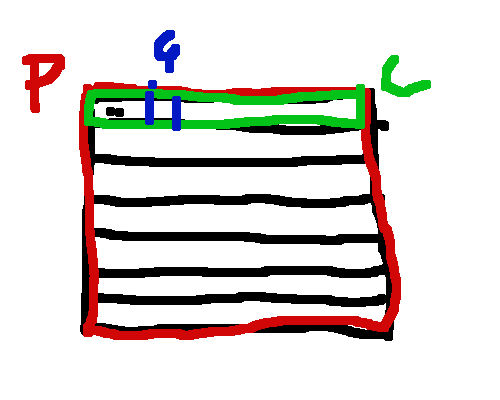
\includegraphics[scale=1.0]{images/Population_Chromosom_Gen.png}
    \caption{Gen, Chromosom und Population}
    \label{fig:population_chromosome_gene}
\end{figure}

Die \textbf{fitness} eines Chromosoms ist der Wert der Zielfunktion für den Phenotyp des Chromosoms. Also der Wert der Zielfunktion für die Parameter welche die Gene des Chromosoms representieren.

\subsection{Ablauf eines genetischen Algorithmus}
Der Ausgangspunkt eines genetischen Algorithmus ist eine Population an Chromosomen. Das erstellen dieser Population nennt man \textbf{Initialisierung}. Gewöhnlicherweise wird die initiale Population zufällig gewählt. Ein Iterationsschritt des klassischen genetischen Algorithmus besteht aus Vier Schritten \cite*{GeneticAlgorithms}.
\begin{itemize}
    \item Selektion: Aus der Population wird eine Menge an Eltern gewählt
    \item Crossover: Die Eltern werden zu einer Menge an Kindern Kindern kombiniert. Typischerweise erzeugen zwei Eltern-Chromosome ein Kind-Chromosom
    \item Mutation: Die Nachkommen werden mutiert, also zufällig verändert
    \item Evaluation: Jedem Kind wird ein fitness-Wert durch die fitness-Funktion zugewiesen
    \item Ersetzung: Die Alte Generation wird durch die neue ersetzt
\end{itemize}
Der Algorithmus terminiert wenn die vorher spezifizierte Anzahl an Generationen erreicht wurde. Alternative Terminierungskriterien sind zum Beispiel maximale Laufzeit des Algorithmus oder maximale Anzahl an Generationen ohne Verbesserung \cite*{TerminologiesAndOperators}. In Figur \ref*{fig:genetic_algorithm_flowchart} wird der beschriebene Ablauf als Flussdiagramm dargestellt.
\begin{figure}[h!]
    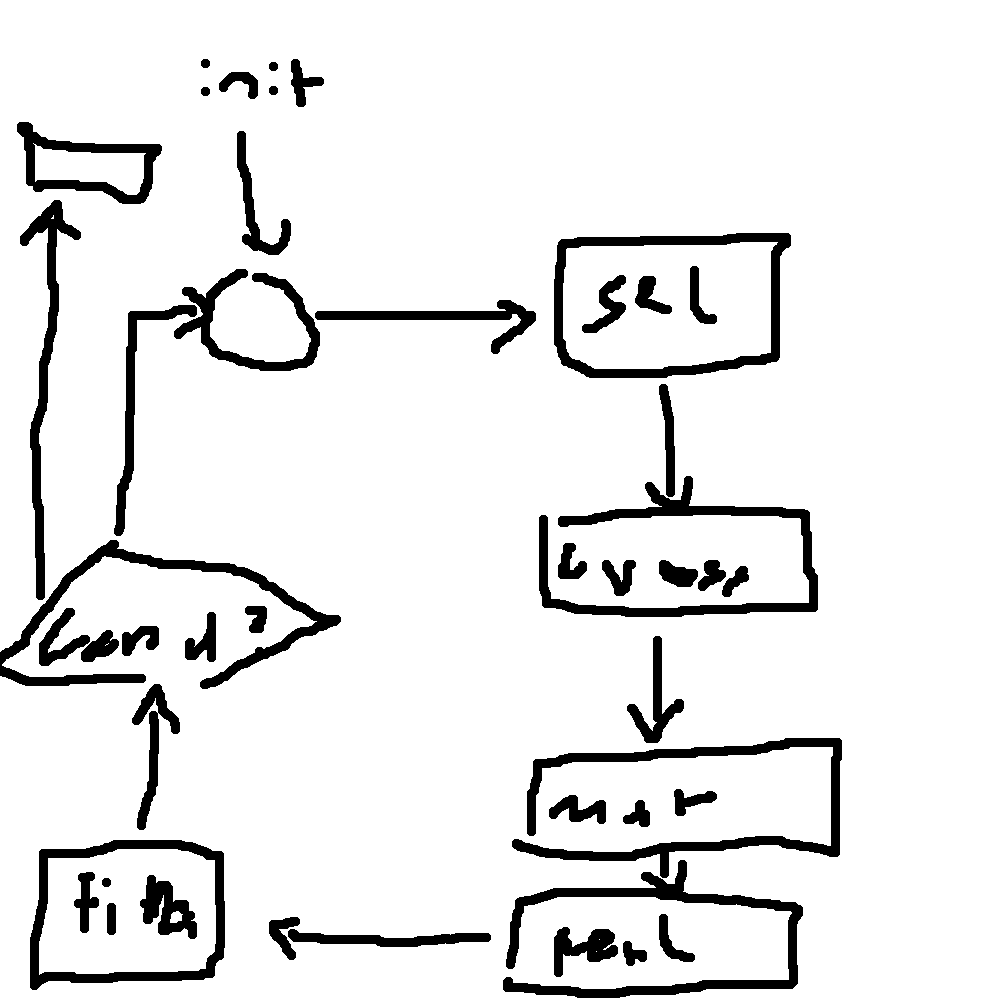
\includegraphics[scale=1.0]{images/Genetic_Algorithm_Flowchart.png}
    \caption{Flussdiagram eines genetischen Algorithmus}
    \label{fig:genetic_algorithm_flowchart}
\end{figure}


\subsection*{Selektionsoperator}
Der Selektionsoperator wählt eine Menge von Eltern aus welchen Kinder für die nächste Generation erzeugt werden. Ganz nach der Evolutionstheorie sollen hier Chromosome mit einer höheren Fitness auch eine höhere Chance haben als Elternteil gewählt zu werden. Wie stark Chromosome mit einer höheren Fitness bevorzugt werden wird als \textbf{Selektionsdruck} bezeichnet. Selektionsstrategien können in zwei Klassen unterteilt werden, \textbf{proportionale Selektion} und \textbf{ordinale Selektion}.~\cite*{TerminologiesAndOperators} Eine proportionale Selektion gewichtet Chromosome anhand ihrer Fitness. Ordinale Selektion gewichtet Chromosome anhand ihres Ranges. Bei einer proportionalen Selektion ist der Selektionsdruck hoch und es besteht das Risiko einer verfrühten Konvergenz. Denn wenn ein einzelnes Chromosom weitaus fitter, als der Rest der Population ist, wird dieses Chromosom einen proportionalen Selektionsprozess dominieren und somit die genetische Diversität der Population senken. Andererseits führt ein geringer Selektionsdruck zu langsamer konvergenz.~\cite{TerminologiesAndOperators} Die Auswahl des Selektionsoperators sollte also wohlüberdacht sein.

\paragraph*{Zufällige Selektion} funktioniert genau so wie der Name vermuten lässt. Die Eltern-Chromosome werden zufällig aus der Population gewählt so dass jedes Chromosom die gleiche Wahrscheinlichkeit hat als Elternteil gewählt zu werden.

\paragraph*{Roulette Rad Selektion} ist einer der traditionellen proportionalen Selektionsoperatoren. Stellen wir uns ein Roulette Rad vor, welches in $N$ Segmente unterteilt ist, wobei $N$ die Anzahl der Chromosome in einer Population ist. Die Länge eines Segmentes $s_i$ ist proportional zu der normalisierten Fitness des korrespondierenden Chromosoms.
\begin{equation}
    s_i = 2 \pi \cdot \frac{fitness(i)}{\sum_{j=1}^{N} fitness(j)}
\end{equation}
Nun wird das Roulette Rad gedreht und das Chromosom auf wessen Feld man landet wird in die Menge der Eltern aufgenommen. Diese Prozedur wird so oft wiederholt bis man die gewünschte Anzahl an Eltern gesammelt hat.

\paragraph*{Rang Selektion} ist eine Abwandlung der Roulette Rad Selektion. Die länge eines Segmentes ist jedoch nicht proportional zu der fitness sondern proportional zu dem Rang des Chromosoms.
\begin{equation}
    s_i = 2 \pi \cdot \frac{N - rank(i)}{\sum_{j=1}^{N} rank(j)}
\end{equation}
Dadurch ist das Risiko einer verfrühten Konvergenz geringer als bei einer Roulette Rad Selektion.
\begin{figure}[h!]
    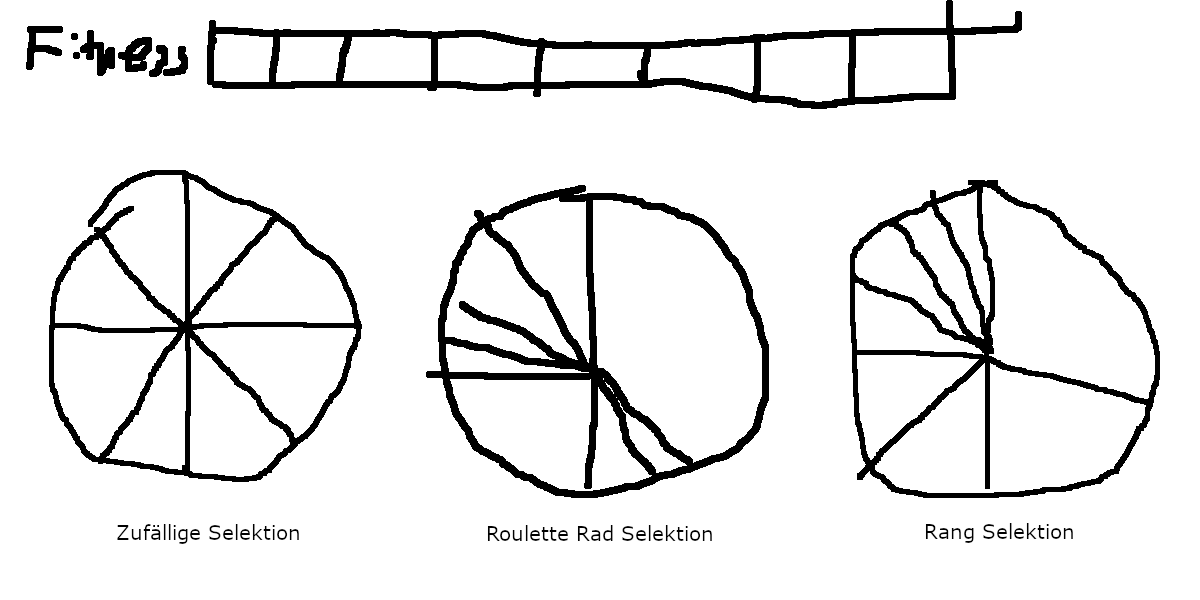
\includegraphics[scale=1.0]{images/Selection_Methods.png}
    \caption{Verschiedene Selektionsoperatoren}
    \label{fig:selection_operators}
\end{figure}

Bei keinem der Selektionsoperator ist garantiert, dass die Chromosome mit der höchsten Fitness als Eltern ausgewählt werden. Darüber hinaus kann es vorkommen, dass Chromosome mit hoher Fitness durch Crossover und Mutation verschlechtert werden, so dass die maximale Fitness der folgenden Generation geringer als die vorherigen ist. Um eine Abnahme der maximalen Fitness zu verhindern wird \textbf{Elitismus} angewendet. Elitismus bedeutet dass einigie der besten Chromosome einer Population, die sogenannten Eliten in jedem Fall in die nächste Generation aufgenommen werden, ohne durch Crossover und Mutation verändert zu werden. Die Anzahl der Eliten ist variabel, um eine Abnahme der maximalen Fitness zu verhindern genügt es aber das Chromosom mit der höchsten Fitness zu übernehmen (Also ein Elitismus von 1).

\subsection{Crossoveroperator}
Als Crossover bezeichnet man das Rekombinieren von typischerweise zwei Eltern-Chromosomen zu einem Kind-Chromosom. Es existieren auch Crossover-Operatoren, welche mehr als zwei Eltern akzeptieren oder mehr als ein Kind produzieren, diese werden wir jedoch nicht betrachten.

Beim \textbf{Single Point Crossover} wird ein Cutpoint entlang der länge der Eltern gewählt. Beide Eltern werden dann an diesem Cutpoint geschnitten und das Kind-Chromosom setzt sich zusammen aus der ersten Hälfte des ersten Elternteils und der zweiten Hälfte des zweiten Elternteils.

\textbf{N-Point Crossover} ist eine Generallisierung des Single Point Crossovers. Es werden $n$ Crossover Points entlang der Länge der Eltern gewählt. Anhand dieser Crossover Points werden die Eltern in $n+1$ Segmente unterteilt. Das Kind erhält alle Segmente mit geradem Index vom ersten Elternteil und alle Segmente mit ungeradem Index vom zweiten Elternteil. Im Allgemeinen führen mehr cutpoints jedoch zu einer geringeren Effizienz  des genetischen Algorithmus.~\cite*{TerminologiesAndOperators}

Bei einem \textbf{uniformen Crossover} wird eine Crossovermaske $m$ mit gleicher Länge zu den Eltern erstellt. Das Kind erhält Gene der Eltern nach dieser Crossover Maske, wobei $m_i$ angibt, von welchem Elternteil das $i$-te Gen bezogen wird. Für jedes Elternpaar wird eine neue Crossovermaske erstellt. Typischerweise gilt $P(m_i = 1) = P(m_1 = 0) = 0.5$. Die Wahrscheinlichkeit, dass ein Gen von einem Elternteil bezogen wird kann jedoch auch gewichtet werden anhand der Fitness oder Ränge, so dass $P(m_i = 0) = w$ und $P(m_i = 1) = 1 - w$

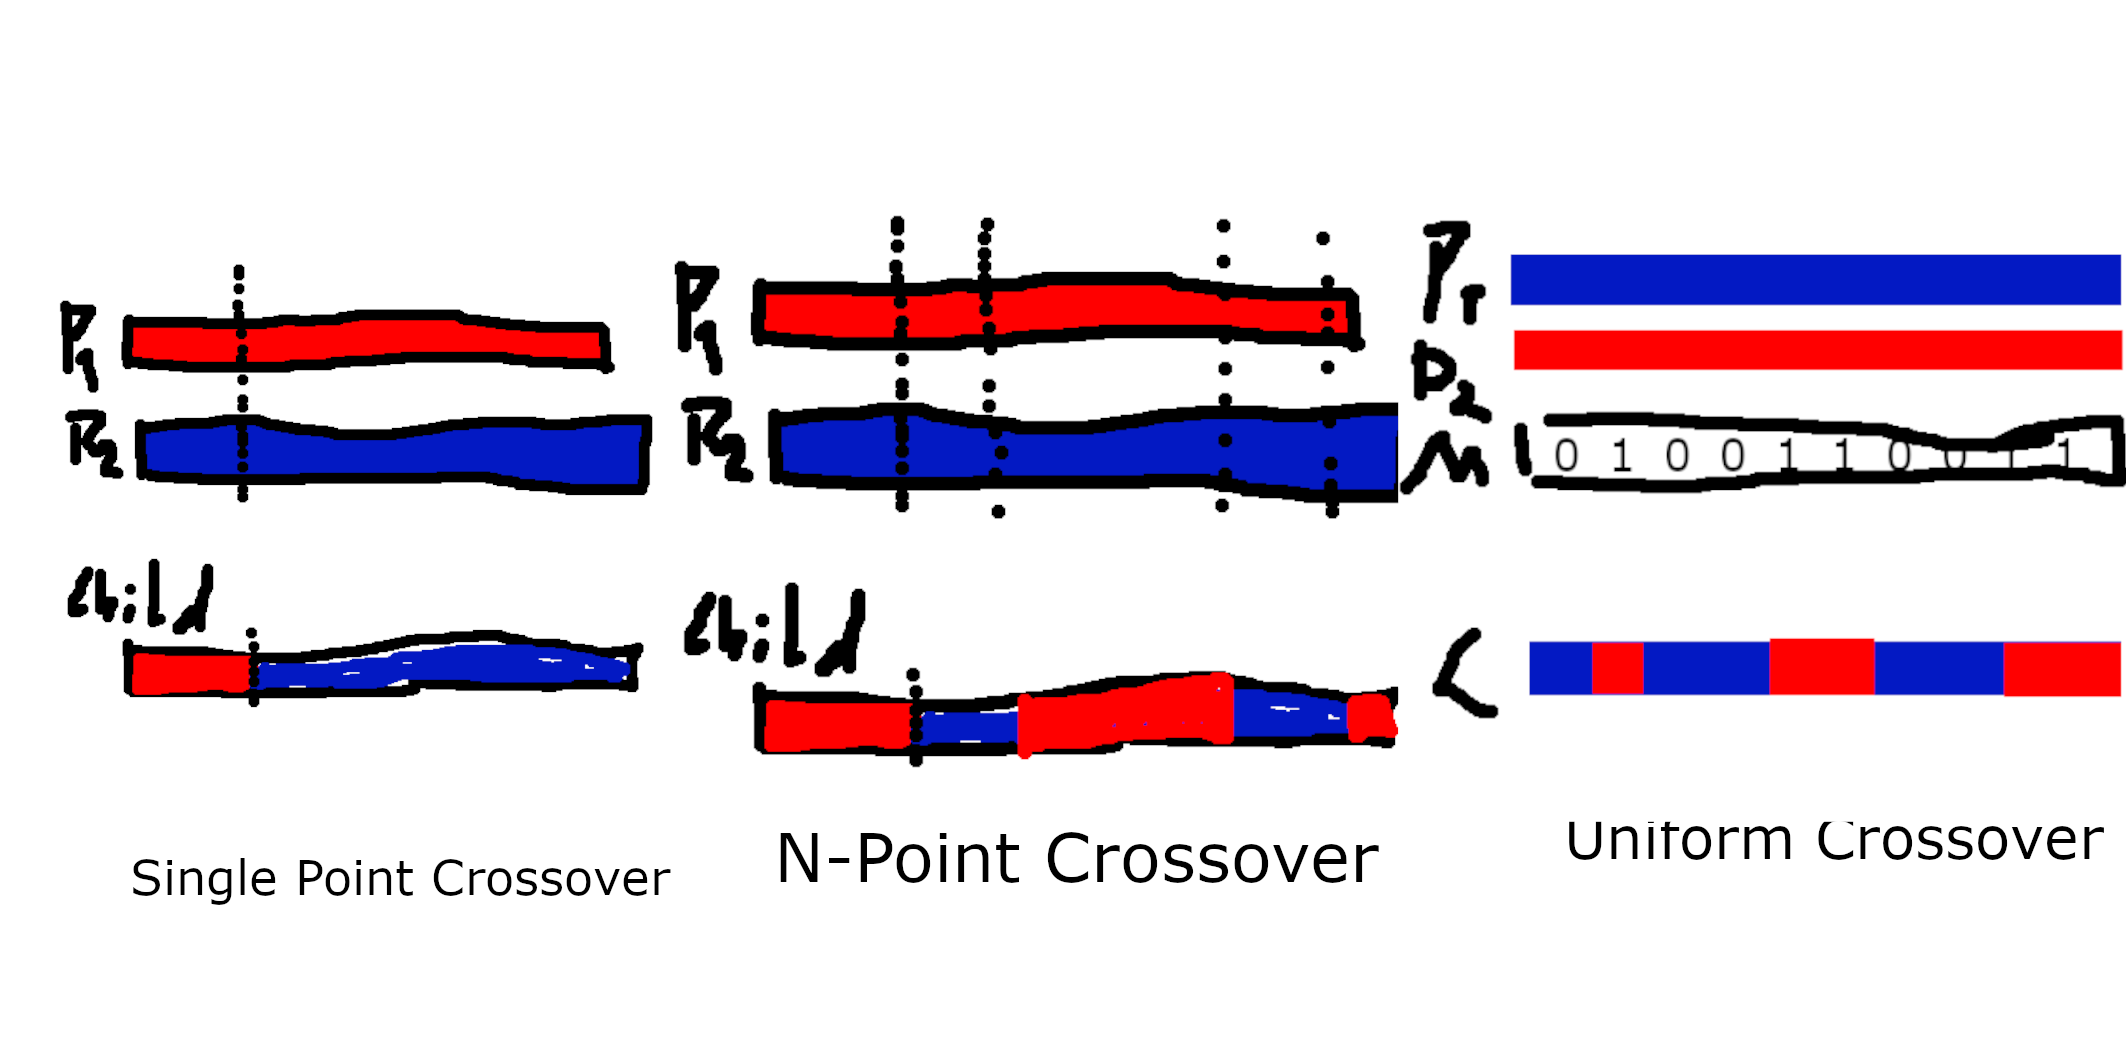
\includegraphics[scale=1.0]{images/Crossover_Methods.png}

Mit der \textbf{Crossover-Wahrscheinlichkeit} kann man festlegen mit welcher Wahrscheinlichkeit ein Crossover zwischen zwei Eltern stattfindet. Für jedes Elternpaar wird eine zufällige Wahrscheinlichkeit generiert. Falls diese Wahrscheinlichkeit größer als die Crossover-Wahrscheinlichkeit ist findet kein Crossover statt und das Kind ist eine exakte Kopie eines Elternteils. So kann man festlegen wie viel genetische Information in der nächsten Generation erhalten bleibt.

\subsection{Mutationsoperator}
Das mehrfache Anwenden von Crossover und Selektion verringert unweigerlich die genetische Diversität der Population. Um dem entgegenzuwirken muss es einen Mechanismus geben, welcher neues genetisches Material hinzufügt. Dieser Mechanismus ist die Mutation, welche ein Chromosom zufällig verändert. Mutation garantiert, dass der Suchraum des genetischen Algorithmus \textbf{ergodisch} ist, was bedeutet das jeder Punkt im Suchraum von jedem anderen erreichbar ist \cite*{TerminologiesAndOperators}. Welche Mutationsoperatoren man verwendet hängt stark vom Problem und der Kodierung eines Chromosoms ab, da viele Mutationsoperatoren nur für bestimmte Arten von Genen anwendbar sind. Ein Bitflip Mutationsoperator zum Beispiel funktioniert logischerweise nur für eine binäre Kodierung. Für diese Arbeit interessieren uns nur Mutationsoperatoren die mit Fließkommazahlen arbeiten.

Die \textbf{Mutationsrate} bestimmt wie viele Gene eines Chromosoms durch die Mutation verändert werden und wie viele Unverändert bleiben. Bei einer Mutationsrate von 100\% werden alle Gene eines Chromosoms verändert  und der genetische Algorithmus ist equivalent zu einer zufälligen Suche.~\cite*{TerminologiesAndOperators}. Für die Mutationsrate sollten im Allgemeinen kleine Werte gewählt werden (wie 0.01 oder 0,001). Eine gute Faustregel ist eine Mutationsrate von $\frac{1}{k}$, wobei $k$ die Anzahl der Gene ist \cite*{MetaheuristicsEGT}.

Ein \textbf{N-Point Random Mutation} Operator wählt zufällig $N$ Gene aus die Mutiert werden sollen und ersetzt diese dann durch zufällige Werte.

Bei einer \textbf{Uniform Random Mutation} wird jedes Gen abhängig von der Mutationsrate mutiert.

TODO: Mutation aus ner alternativen Verteilung als Standardverteilung wählen.

\subsection*{Ersetzung}
TODO: Ersetzungsstrategien

\subsection*{Parameter eines genetischen Algorithmus}
Wie im Abschnitt [Abschnitt Label hier] erwähnt haben Metaheuristiken den Nachteil, dass sie neue Parameter einführen. Ein genetischer Algorithmus, wie er zuvor beschrieben wurde hat folgende Parameter.
\begin{enumerate}
    \item Populationsgröße
    \item Anzahl der Generationen (oder Abbruchbedingung)
    \item Mutationsfunktion und Mutationsrate
    \item Crossoverfunktion und Crossoverrate
    \item Selektionsfunktion
    \item Anzahl der Eliten
    \item Ersetzungsstrategie
\end{enumerate}
Die Belegung dieser Parameter ist keinesfalls trivial denn die Parameter beeinflussen die Konvergenzrate des Algorithmus maßgeblich. Die Populationsgröße zum Beispiel beeinflusst die globale Suchkapazität, ein größerer Wert ist hier von Vorteil. Jedoch benötigt eine große Populationi auch mehr Rechenleistung, Speicher und Zeit \cite*{TerminologiesAndOperators}. Die Mutationsrate beeinflusst ebenfalls die Konvergenzrate. Eine zu hohe Mutationsrate führt zu einer langsamen Konvergenz und einem ineffizienten Algorithmus. Eine zu niedrige Mutationsrate führt wiederum zu einer verfrühten Konvergenz und somit zu weniger optimierten Lösungen. Die Auswahl der genetischen Operatoren wirkt sich unter anderem auf die Rechenlast aus. Ein Single-Point-Crossover zum Beispiel generiert eine zufällige Zahl, und macht einen Vergleich. Die Anzahl der benötigten Zufallszahlen und Vergleiche bei einem Uniform-Crossover hingegen sind equivalent zu der Anzahl an Genen. Bei mehreren Hunderten von Genen macht sich dieser Unterschied durchaus bemerkbar.